\documentclass[11pt,a4paper]{article}
\usepackage[margin=25mm]{geometry}
\usepackage[T1]{fontenc}
\usepackage{lmodern}
\usepackage{microtype}
\usepackage{booktabs}
\usepackage{graphicx}
\usepackage{subcaption}
\usepackage{amsmath}
\usepackage{amssymb}
\usepackage{siunitx}
\usepackage{hyperref}
\usepackage{float}
\usepackage{longtable}
\hypersetup{colorlinks=true,linkcolor=blue,citecolor=blue,urlcolor=blue}
\graphicspath{{figures/}}
\title{Prediction of Myocardial Infarction Complications with\\Admission-Time Clinical Data}
\author{Student report draft}
\date{\today}
\begin{document}
\maketitle
\begin{abstract}
This report documents a reproducible machine-learning workflow for separate prediction of in-hospital death, heart failure (ZSN), and post-infarction fibrillation (FIBR\_PREDS) in the myocardial infarction complications dataset. Development-only cross-validation informed target-specific model selection and Platt calibration. A single approved evaluation of the frozen models was made on the fixed 20\% test partition. The test results are reported separately from development estimates. This is a first draft: six assignment question responses remain explicit student placeholders.
\end{abstract}
\tableofcontents
\section{Introduction and objectives}
Acute myocardial infarction (MI) is associated with complications that can change rapidly during hospitalization. This project applies supervised learning to admission-time clinical variables to estimate three outcomes separately: death (the assignment's \texttt{LET\_IS} probability), heart failure (\texttt{ZSN}), and fibrillation (\texttt{FIBR\_PREDS}). The assignment emphasizes useful probability estimates and careful validation, rather than accuracy alone \cite{assignmentguide,ucimi}.

The objectives were to establish prevalence and regularized-logistic baselines; compare tree ensembles using development-only cross-validation; select a frozen model, calibrator, and operating threshold for each outcome; assess the frozen system once on the locked test partition; and explain the mortality model using SHAP. This report is a first draft. The six required written question responses are left for the student in Section~\ref{sec:questions}.

\section{Dataset, outcomes, and preprocessing}
The project uses the UCI Myocardial Infarction Complications dataset, a retrospective clinical dataset containing admission characteristics and outcomes \cite{ucimi}. The source file and variable dictionary are retained in the project; Stage~1 outputs supply the development/test partitions, predictor tables, and role documentation. The available project summary records 1,700 admissions: 1,360 development records and 340 held-out records. Development mortality prevalence is 15.96\%; test mortality prevalence is 15.88\% as recorded in the split summary and aggregate T07 report.

The targets are treated as separate binary tasks. Death is defined as $\mathbb{1}(\texttt{LET\_IS}>0)$ and the held-out evaluator checks consistency with that definition. Predictors exclude IDs, all outcome columns, and the documented post-admission fields. The feature matrices are the existing Stage~1 tables; downstream stages do not reconstruct the split.

Preprocessing is estimator-specific. Random Forest pipelines perform fold-local median numeric and mode categorical imputation followed by one-hot encoding for nominal features. The selected CatBoost model uses native categorical features and its supported numeric missing-value behavior, with categorical missingness represented by the training pipeline's sentinel convention. No class weighting or resampling was used for the frozen finalists; probabilities therefore reflect natural development prevalence. Learned preprocessing is fitted within training folds, not before cross-validation. Full detail and feature roles are in \texttt{mi\_stage1\_eda.py}, \texttt{mi\_column\_dictionary.csv}, and the Stage~1/5 audit outputs.

\subsection{Split and validation design}
Stage~1 fixes a stratified 80/20 split using random seed 42, stratified on \texttt{DEATH\_BINARY}. This yielded 1,360 development and 340 test records. Development model comparisons use five stratified folds with seed 42 and target-specific eligible rows. Average precision (AP, equivalent to non-interpolated area under the precision-recall curve in these reports) is the primary ranking/tuning criterion; AUROC, Brier score, and log loss are secondary. The Stage~6 report checks fold signatures against preceding stages. Test labels were not used for model or threshold selection. The final frozen model, calibrator, and threshold were fixed in T06 before the single T07 test evaluation.

\section{Comparable development cross-validation and model selection}
Table~\ref{tab:cv} summarizes the required prevalence baseline, regularized logistic regression, and the target-specific tree model ultimately frozen in T06. Values are Stage~6 common-fold means and sample standard deviations on development data. They are not held-out test results and are descriptive rather than significance tests. The full seven-model comparison is in \texttt{stage6\_catboost\_outputs/stage6\_report.md}; Figure~\ref{fig:cv} shows that broader comparison.

\begin{table}[H]
\centering\small
\caption{Comparable development CV results (mean $\pm$ sample SD, five folds).}\label{tab:cv}
\begin{tabular}{llrrr}\toprule
Target & Model & AP & AUROC & Brier\\\midrule
Death & Dummy prior & $0.160\pm0.002$ & $0.500\pm0.000$ & $0.134\pm0.001$\\
Death & Logistic regression & $0.651\pm0.031$ & $0.879\pm0.017$ & $0.089\pm0.005$\\
Death & CatBoost tuned & $0.733\pm0.059$ & $0.901\pm0.022$ & $0.077\pm0.009$\\\midrule
ZSN & Dummy prior & $0.225\pm0.002$ & $0.500\pm0.000$ & $0.174\pm0.001$\\
ZSN & Logistic regression & $0.315\pm0.030$ & $0.621\pm0.025$ & $0.179\pm0.005$\\
ZSN & Random Forest tuned & $0.502\pm0.083$ & $0.718\pm0.045$ & $0.148\pm0.013$\\\midrule
FIBR\_PREDS & Dummy prior & $0.099\pm0.000$ & $0.500\pm0.000$ & $0.089\pm0.000$\\
FIBR\_PREDS & Logistic regression & $0.246\pm0.068$ & $0.702\pm0.071$ & $0.089\pm0.008$\\
FIBR\_PREDS & Random Forest preliminary & $0.301\pm0.108$ & $0.725\pm0.063$ & $0.083\pm0.005$\\\bottomrule
\end{tabular}
\end{table}
\begin{figure}[H]\centering
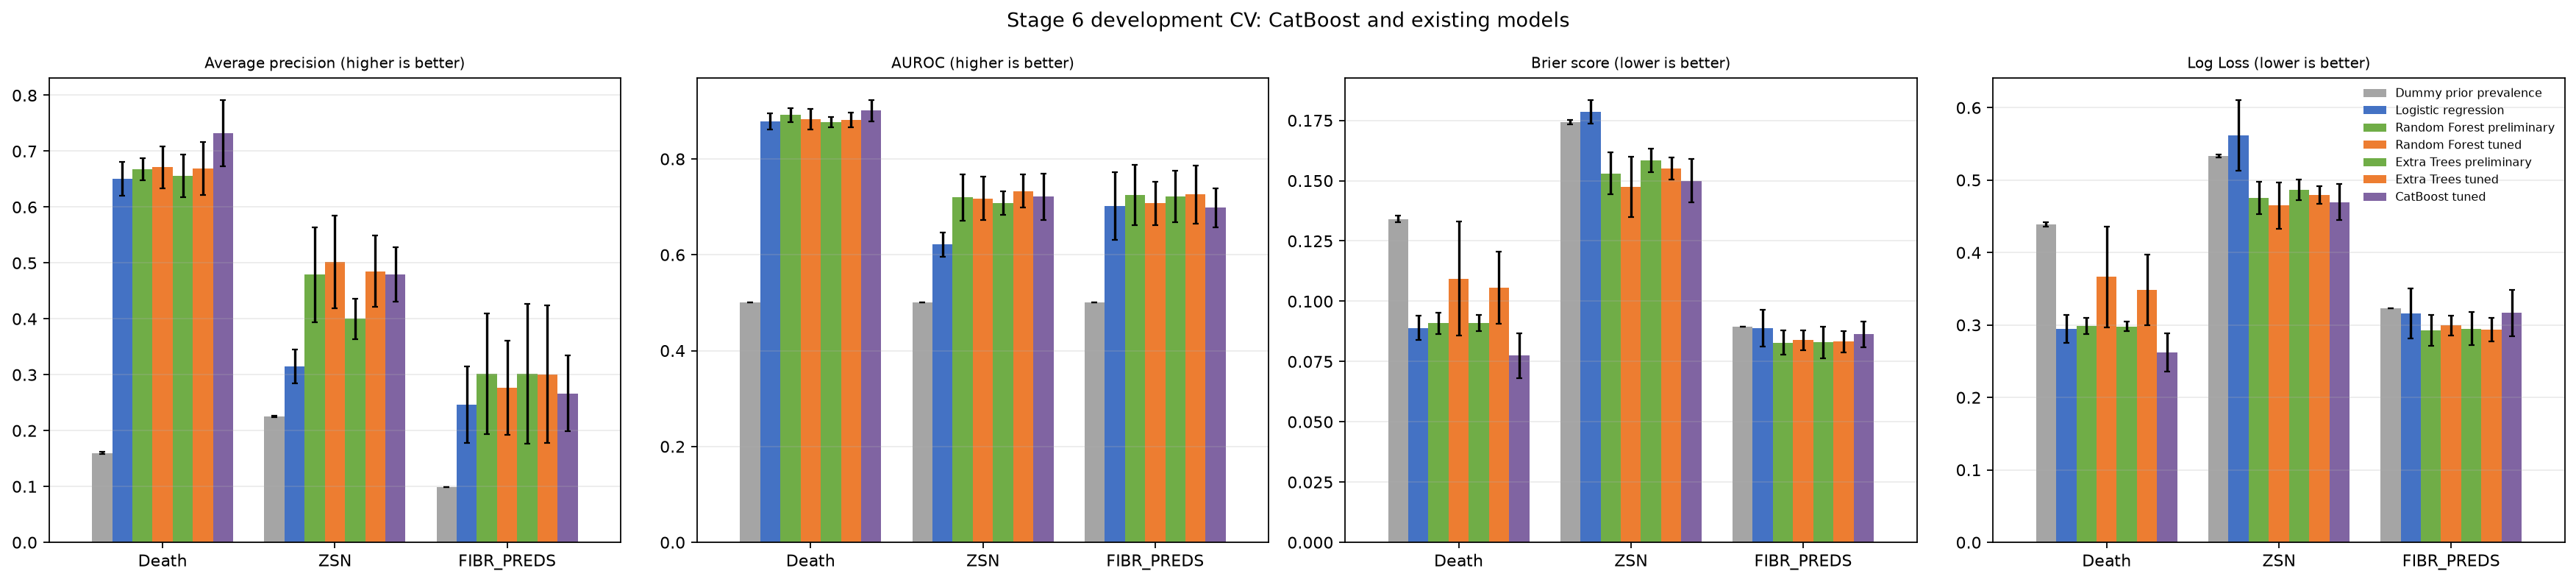
\includegraphics[width=.98\linewidth]{model_comparison.png}
\caption{Stage~6 common-fold comparison across the existing model candidates. Source: \texttt{stage6\_catboost\_outputs/model\_comparison.png}.}\label{fig:cv}
\end{figure}

T06 froze CatBoost tuned for mortality, tuned Random Forest for ZSN, and preliminary Random Forest for fibrillation. Mortality CatBoost had the strongest saved mean AP among the compared candidates (0.7326 versus 0.6713 for tuned RF) and better mean AUROC/Brier evidence. For ZSN, tuned RF had the strongest saved AP (0.5018); Extra Trees tuned was the nearest alternative at 0.4850. For FIBR\_PREDS, preliminary RF and Extra Trees were effectively tied in AP (0.301054 versus 0.301365, gap 0.000311, smaller than either fold SD); RF was retained as a balanced choice because its saved mean AUROC was slightly higher and its Brier/log loss slightly lower. The final manifest identifies these as revision \texttt{non\_tabpfn\_v1}. This selection did not use test outcomes.

\section{Probability calibration}
The frozen approach applies Platt (sigmoid) calibration to each model. In T06, base predictions were cross-fitted on development folds; each outer training partition generated inner out-of-fold scores for calibration, and the outer validation fold did not fit its model or calibrator. The final bundle fits the Platt mapping to fresh cross-fitted development scores and refits the base estimator on eligible development rows. Thresholds maximize specificity subject to a development sensitivity constraint of at least 0.80; this is a prespecified operating-point assumption, not a universal clinical threshold. Thresholds are 0.15333596 (death), 0.16286458 (ZSN), and 0.07103629 (FIBR\_PREDS). No threshold is used in the probability export.

Table~\ref{tab:development-cal} compares raw and fold-local Platt probabilities on the same 1,360 outer-OOF development records. Platt improved Brier and log loss slightly for death and ZSN; for FIBR\_PREDS both worsened slightly, while Platt remained the frozen assignment-required calibration method. These are development metrics, not test metrics.
\begin{table}[H]\centering\small
\caption{Development OOF probability scores before and after fold-local Platt calibration.}\label{tab:development-cal}
\begin{tabular}{lrrrr}\toprule
Target & Raw Brier & Platt Brier & Raw log loss & Platt log loss\\\midrule
Death & .077211 & .074604 & .262351 & .253899\\
ZSN & .147352 & .146906 & .466140 & .464788\\
FIBR\_PREDS & .082854 & .083415 & .292421 & .294540\\\bottomrule
\end{tabular}\end{table}

The reliability plots in Figure~\ref{fig:devcal} use T06 outer OOF development predictions and quantile bins; they visualize raw versus fold-local Platt scores. Figure~\ref{fig:testcal} is separate and shows the frozen Platt predictions on the final test partition. T07 reports ten-bin equal-width ECE, along with descriptive joint calibration intercept/slope; none of these test diagnostics refits the frozen calibrator.
\begin{figure}[H]\centering
\begin{subfigure}{.32\linewidth}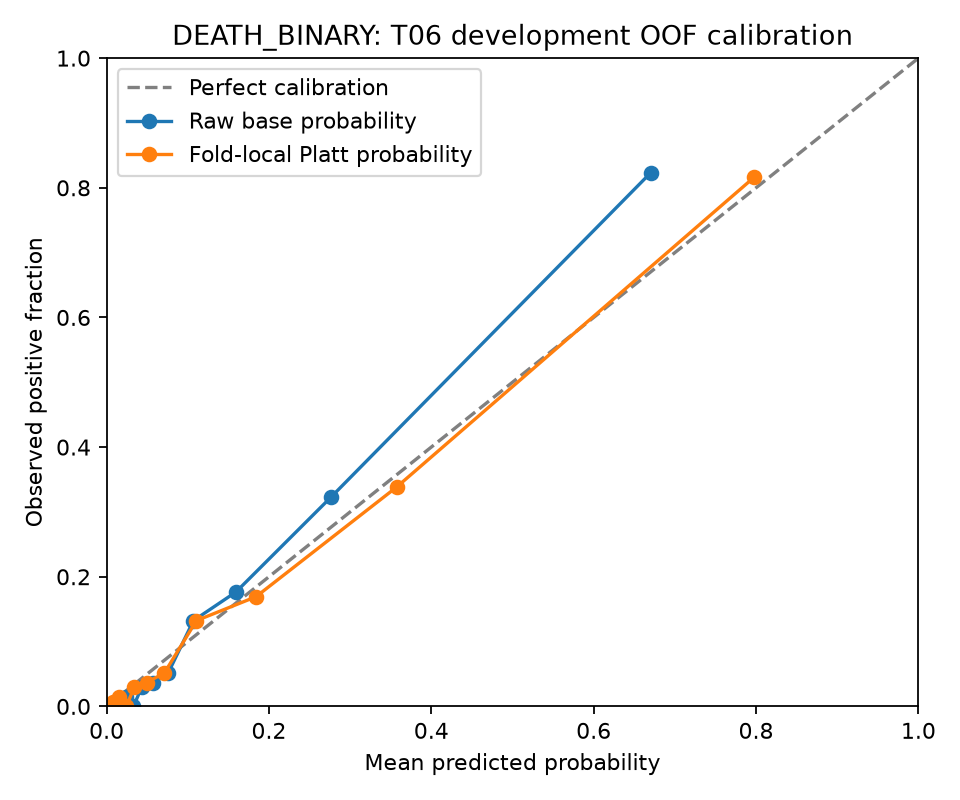
\includegraphics[width=\linewidth]{development_death_binary_raw_vs_platt_reliability.png}\caption{Death}\end{subfigure}
\begin{subfigure}{.32\linewidth}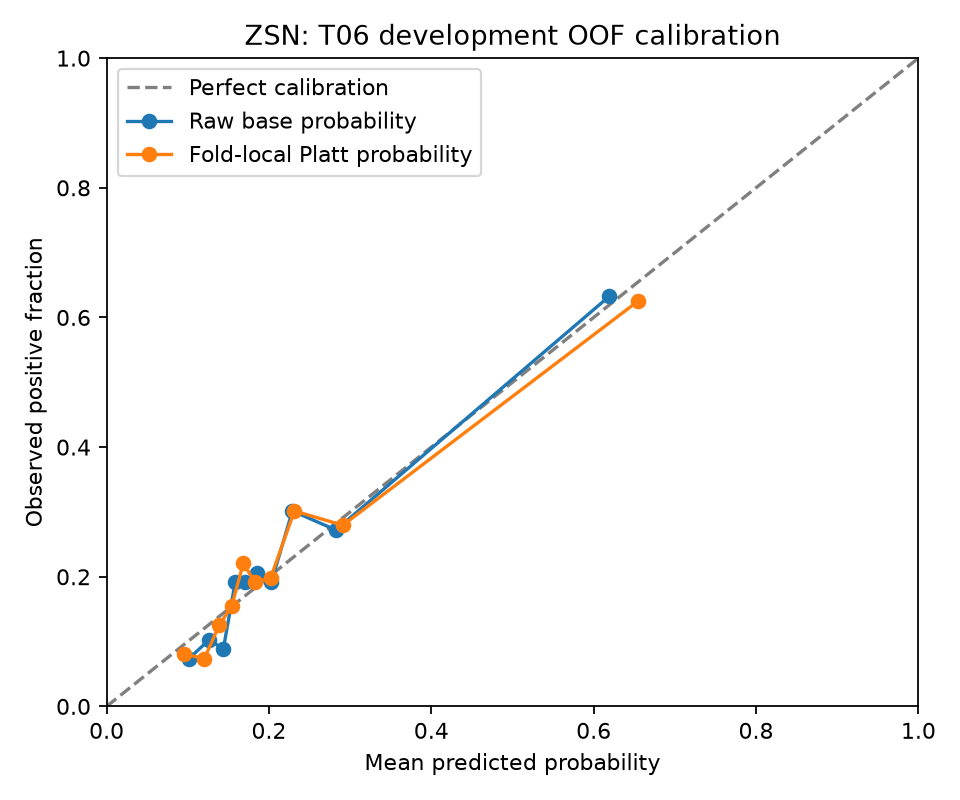
\includegraphics[width=\linewidth]{development_zsn_raw_vs_platt_reliability.png}\caption{ZSN}\end{subfigure}
\begin{subfigure}{.32\linewidth}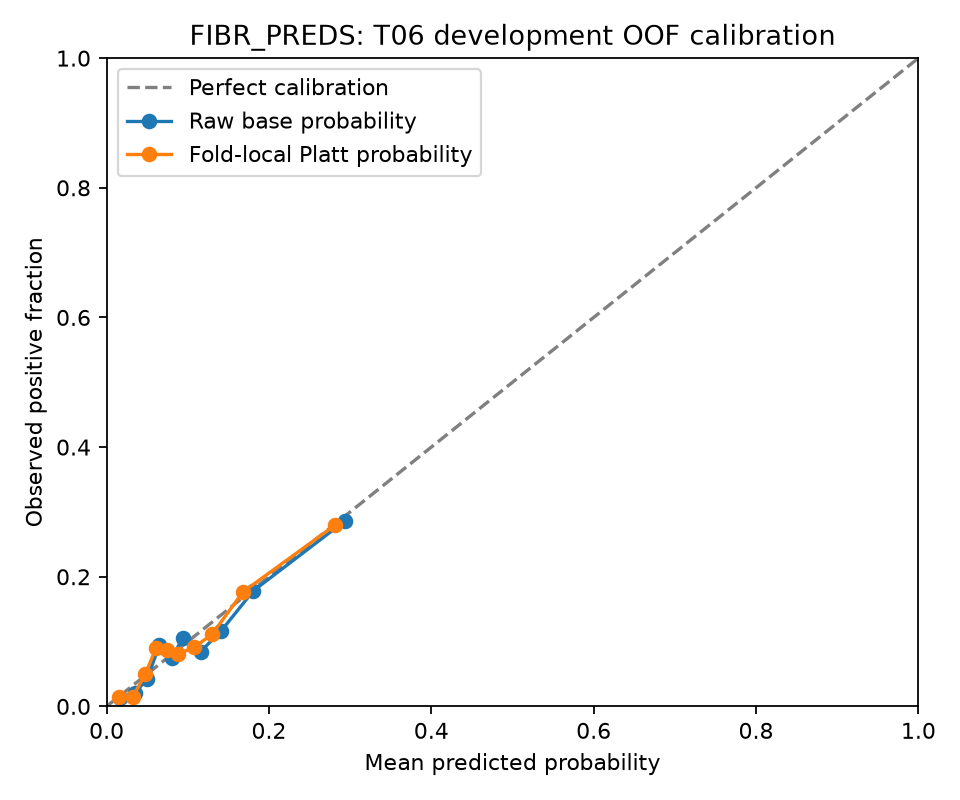
\includegraphics[width=\linewidth]{development_fibr_preds_raw_vs_platt_reliability.png}\caption{FIBR\_PREDS}\end{subfigure}
\caption{Development outer-OOF reliability comparisons. Source: T07 development comparison plots, based on T06 OOF data.}\label{fig:devcal}
\end{figure}

\section{Final held-out evaluation}
After the T06 freeze and reported TA authorization, T07 evaluated the three frozen bundles once on the 340-record Stage~1 test partition. The evaluator used saved features, outcomes, and IDs in their existing row order; no tuning or refitting used test labels. Ranking, calibration, and threshold metrics are reported separately. Table~\ref{tab:test-rank} includes seeded percentile paired-row-bootstrap 95\% intervals (1,000 replicates, seed 42); Table~\ref{tab:test-cal} presents probabilities; Table~\ref{tab:test-threshold} gives confusion matrices at the frozen development thresholds.

\begin{table}[H]\centering\small
\caption{Held-out ranking results and bootstrap 95\% confidence intervals.}\label{tab:test-rank}
\begin{tabular}{lrrr}\toprule
Target & AUROC (95\% CI) & AP (95\% CI) & $n$\\\midrule
Death & .8836 [.8321,.9295] & .7108 [.5927,.8086] & 340\\
ZSN & .7266 [.6605,.7859] & .5957 [.4996,.6814] & 340\\
FIBR\_PREDS & .6567 [.5518,.7624] & .1919 [.1180,.3218] & 340\\\bottomrule
\end{tabular}\end{table}

\begin{table}[H]\centering\small
\caption{Held-out probability and calibration metrics for frozen Platt probabilities. Brier baseline uses observed test prevalence.}\label{tab:test-cal}
\begin{tabular}{lrrrrrr}\toprule
Target & Brier & Baseline & BSS & Log loss & ECE & Intercept / slope\\\midrule
Death & .0799 & .1336 & .4021 & .2680 & .0256 & $-.0365/1.0103$\\
ZSN & .1538 & .1918 & .1983 & .4811 & .0438 & $.7212/1.4001$\\
FIBR\_PREDS & .0900 & .0923 & .0258 & .3222 & .0273 & $-.8126/.6032$\\\bottomrule
\end{tabular}\end{table}

\begin{table}[H]\centering\scriptsize
\caption{Held-out classification at frozen T06 thresholds; confusion counts are TN/FP/FN/TP.}\label{tab:test-threshold}
\begin{tabular}{lrrrrrrr}\toprule
Target & Threshold & Sens. & Spec. & Precision & F1 & Accuracy & TN/FP/FN/TP\\\midrule
Death & .153336 & .7593 & .8182 & .4409 & .5578 & .8088 & 234/52/13/41\\
ZSN & .162865 & .7727 & .4444 & .3269 & .4595 & .5294 & 112/140/20/68\\
FIBR\_PREDS & .071036 & .7429 & .4623 & .1368 & .2311 & .4912 & 141/164/9/26\\\bottomrule
\end{tabular}
\end{table}
\noindent Specificity, sensitivity, and accuracy should be interpreted alongside prevalence and ranking/calibration metrics.

\begin{figure}[H]\centering
\begin{subfigure}{.32\linewidth}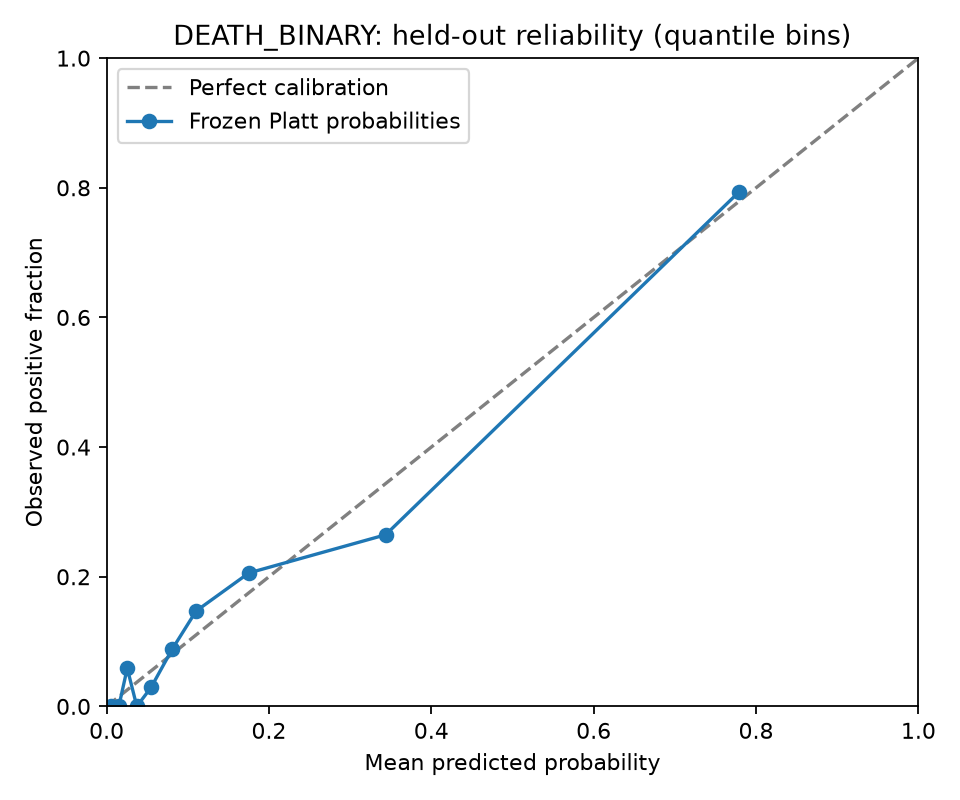
\includegraphics[width=\linewidth]{death_binary_reliability.png}\caption{Death}\end{subfigure}
\begin{subfigure}{.32\linewidth}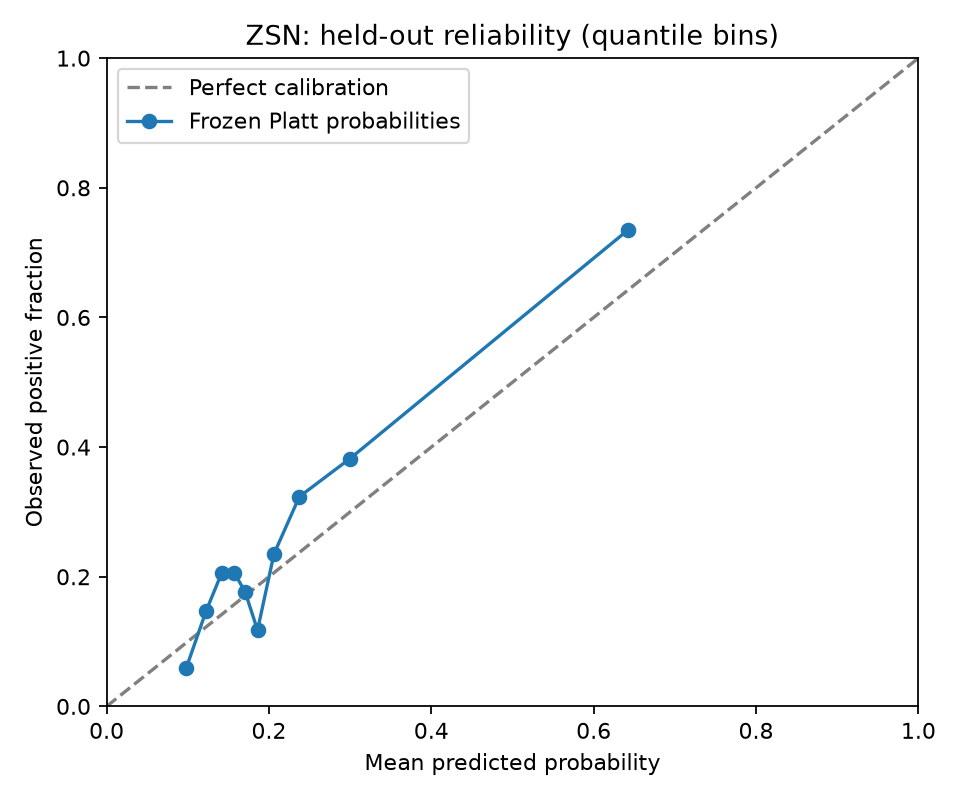
\includegraphics[width=\linewidth]{zsn_reliability.png}\caption{ZSN}\end{subfigure}
\begin{subfigure}{.32\linewidth}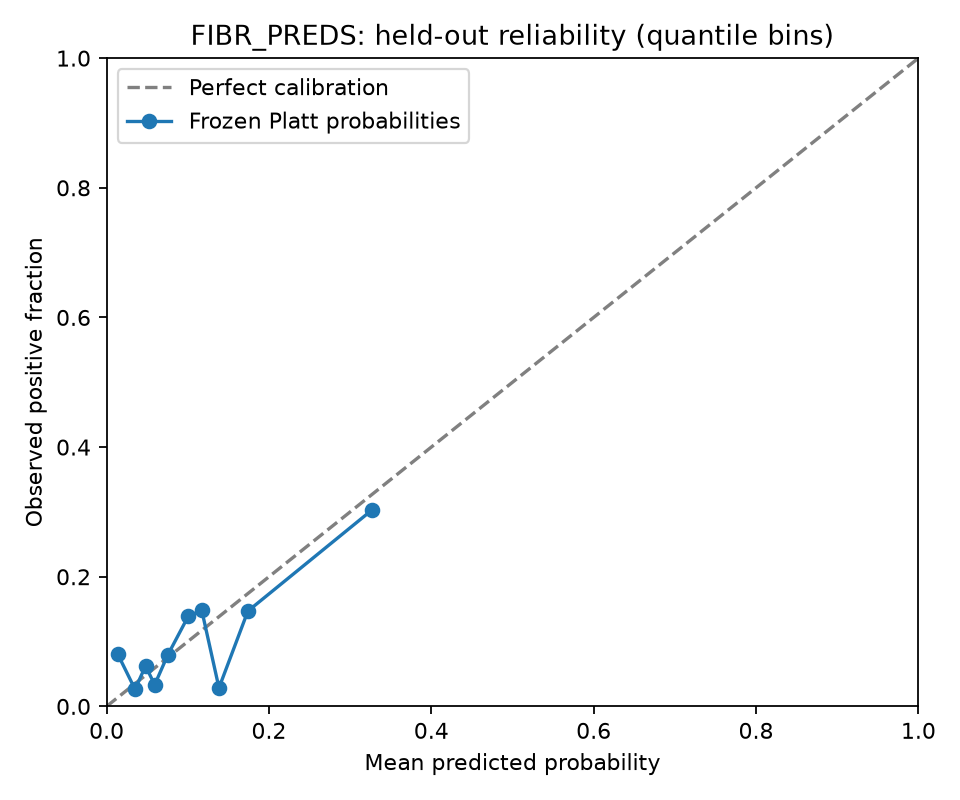
\includegraphics[width=\linewidth]{fibr_preds_reliability.png}\caption{FIBR\_PREDS}\end{subfigure}
\caption{Final test reliability diagrams for the frozen Platt predictions. These are descriptive test-set diagnostics and did not alter predictions. Source: T07 outputs.}\label{fig:testcal}
\end{figure}

The T07 report also provides decision curves from threshold probabilities 0.05--0.40 against treat-all and treat-none strategies. They are descriptive and do not select the frozen operating thresholds. Aggregate numeric results and run provenance are in \texttt{stage11\_t07\_outputs/}; the separate assignment probability export is \texttt{stage12\_t08\_outputs/submission.csv} with header \texttt{ID,LET\_IS,ZSN,FIBR\_PREDS}.

\section{Mortality model explanation with SHAP}
The mortality explanation uses the frozen T06 CatBoost base estimator and development predictors only. Native CatBoost Independent TreeSHAP values were calculated on the 1,360 development rows, with a 64-row development reference sample selected using seed 42. The Platt calibrator and decision threshold were not applied to the attribution values; SHAP explains the model's raw score \cite{lundberg2020,prokhorenkova2018}. Figure~\ref{fig:shap} is the summary plot, where features are ordered by mean absolute contribution. The largest mean absolute attributions were AGE (0.2935), ZSN\_A (0.2911), ant\_im (0.2873), TIME\_B\_S (0.2699), and STENOK\_AN (0.2131). The source dictionary describes them as age, chronic heart failure in the anamnesis, anterior MI ECG pattern, time from attack onset to hospital, and prior exertional angina.

These ranks describe contribution magnitude in this fitted model, not causal effects or a uniform direction of effect. The monochrome plot does not encode feature values. The guide's optional local explanations for two example patients are not supplied in this draft.
\begin{figure}[H]\centering
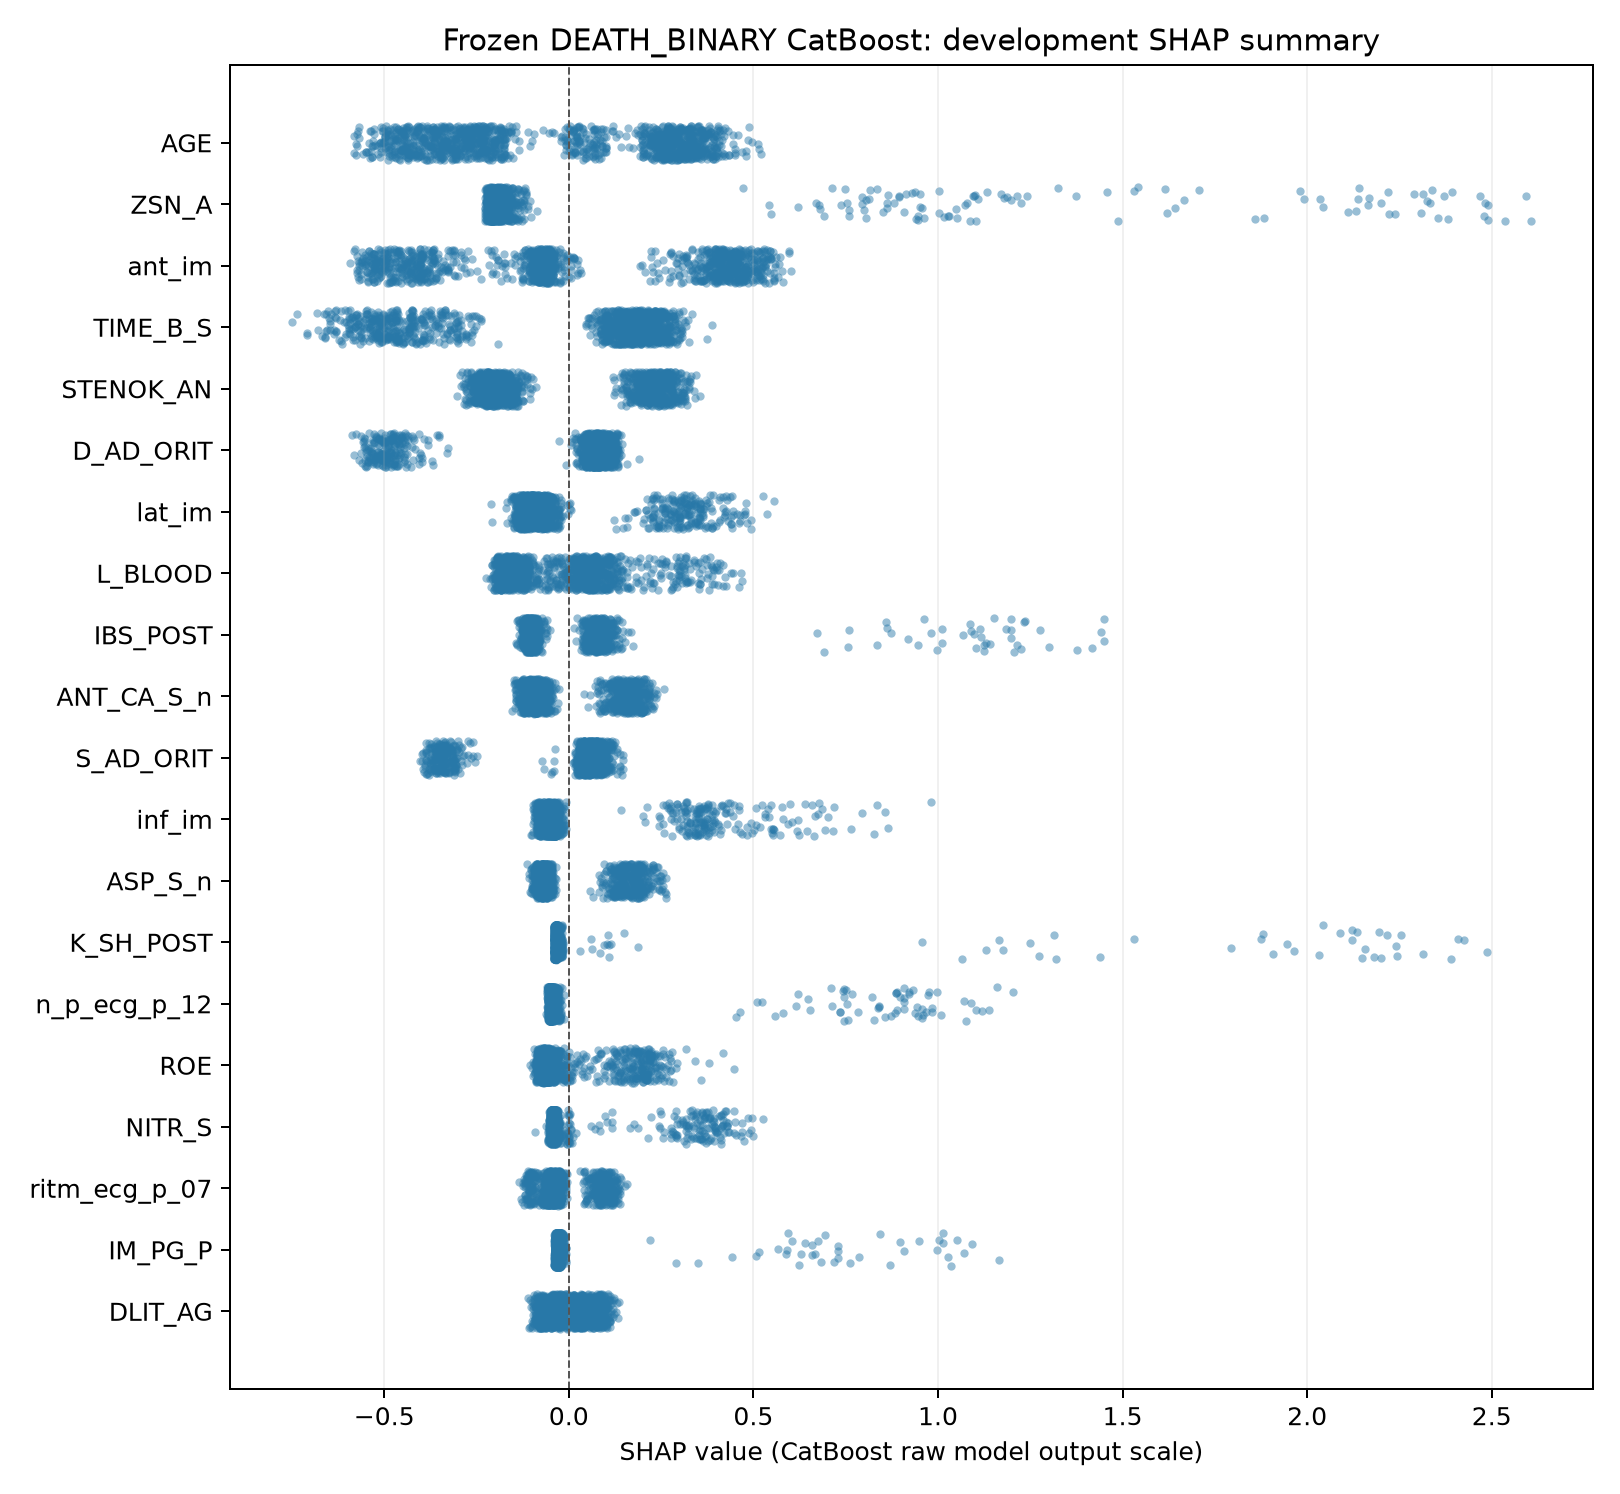
\includegraphics[width=.85\linewidth]{mortality_shap_summary.png}
\caption{Development-only SHAP summary for frozen mortality CatBoost. Source: \texttt{stage13\_t09\_mortality\_shap\_outputs/mortality\_shap\_summary.png}.}\label{fig:shap}
\end{figure}

\section{Assignment questions awaiting student responses}\label{sec:questions}
The assignment requires four experiment-supported answers and two literature-review answers. No response is supplied here. Complete each placeholder using the indicated evidence, and cite the exact analysis/output added to the final submission.

\subsection{Mandatory question 1: leakage and preprocessing}
\textbf{[ANSWER TO BE COMPLETED BY STUDENT]}\par
Required evidence: run a small controlled development-only comparison showing imputation or SMOTE applied before splitting versus fitted/applied inside each training fold. Report fold scores, explain leakage direction, and identify which estimate is trustworthy. Do not use the held-out test set for this experiment.

\subsection{Mandatory question 2: probabilities after 1:1 undersampling}
In five-fold stratified development cross-validation, the observed mortality prevalence across the 1,360 outer-fold predictions was 0.1596. A Stage~2 regularized logistic regression was trained after 1:1 undersampling. For each outer fold, a separate stratified 20\% subset of the outer training data retained its natural prevalence; the base model, fit on the disjoint remaining subset after undersampling, generated scores for this calibration subset. Platt scaling (Section~11.3) was fitted to those held-out scores and labels, then applied to the untouched outer validation fold. No validation labels were used for fitting. The pooled mean predicted mortality probabilities were 0.3411 raw, 0.1768 after the distinct odds-based prior correction, and 0.1663 after Platt calibration. Brier score was 0.1520, 0.0964, and 0.0938, respectively; log loss was 0.4802, 0.3246, and 0.3103; ten-bin quantile ECE was 0.1831, 0.0436, and 0.0123. Platt had the best pooled probability scores and a calibration slope of 1.0116/intercept of -0.0563, though its AUROC (0.8534) was slightly lower than raw/prior correction (about 0.8590). Its mean probability (0.1663) remained slightly above prevalence. The outputs, reliability plot, and run manifest are in \texttt{undersampling\_calibration\_outputs/}; the earlier prior-correction-only experiment is preserved separately. No held-out records were used.

\subsection{Mandatory question 3: asymmetric decision cost}
Using the frozen T06 CatBoost model's Platt-calibrated five-fold outer development OOF probabilities (1,360 patients; observed death prevalence 0.1596), I classify a patient as high risk when $p(\mathrm{death})\ge t$ and minimize empirical cost $10FN+FP$. The threshold grid included zero, every distinct OOF probability, and an all-negative cutoff just above the maximum; ties select the highest threshold. The minimum-cost threshold was $t=0.101369$, with TP=197, FP=305, TN=838, FN=20, and total cost 505. Thus 502 patients were alerted: 36.91 alerts per 100 (369.12 per 1,000). There were 197 deaths identified: 14.49 per 100 (144.85 per 1,000), with 20 deaths missed. Alert rate is alerts divided by all patients, whereas sensitivity is deaths identified divided by actual deaths (0.9078); deaths identified per 100 patients is TP divided by all patients. At $t=0.5$, cost was 1,079; at the existing frozen threshold 0.153336, cost was 636. The selected threshold is an empirical development operating point evaluated on the same OOF records used to optimize it; its apparent cost may be optimistic, so it does not replace the frozen T06 threshold or constitute a final test evaluation. Results and reproducibility details are in \texttt{mi\_cost\_sensitive\_threshold\_outputs\_v2/}.

\subsection{Mandatory question 4: prediction versus causality}
\textbf{[ANSWER TO BE COMPLETED BY STUDENT]}\par
Required evidence: use the guide's heparin example and identify an important feature in the fitted model, then distinguish predictive association from causal effect. Explain confounding, treatment timing, and what causal design or data would be needed. The SHAP results in this report do not establish causality.

\subsection{Literature-review question 1: student-selected guide article}
\textbf{[ANSWER TO BE COMPLETED BY STUDENT]}\par
Select an article and its associated first literature-review prompt from the guide; summarize the study question, cohort, method, principal result, and limitations, with a citation. Article and prompt selection are pending.

\subsection{Literature-review question 2: student-selected guide article}
\textbf{[ANSWER TO BE COMPLETED BY STUDENT]}\par
Select an article and its associated second literature-review prompt from the guide; answer using the paper's evidence and a comparison with this project's task where appropriate. Article and prompt selection are pending; no literature questions have been selected on the student's behalf.

\section{Limitations and reproducibility}
The dataset is retrospective and reflects its source population and measurement practices. Small five-fold samples, especially for the less prevalent outcomes, produce variable estimates; development CV summaries and bootstrap intervals are descriptive, not guarantees of deployment performance. The threshold constraint of 0.80 sensitivity is an operating-point assumption. T06 notes that the full-development estimator is trained on more records than the outer-fold estimators used to produce calibration scores, so calibration transfer can be imperfect. The FIBR\_PREDS Platt mapping slightly worsened development Brier and log loss relative to raw scores, and the held-out FIBR ranking/calibration results are weaker than for the other outcomes.

The most important alignment limitation is preserved from T07: the Stage~1 source uses a shared \texttt{test\_idx} to create X, y, and IDs, and the saved test row count is checked. However, the existing CSVs contain no shared row-level key or alignment fingerprint. Thus exact row-by-row correspondence between saved test predictors and IDs cannot be independently proven from current artifacts. The split was not recreated. This limitation does not change the recorded evaluation, but it should accompany interpretation of row-specific audit outputs.

The T07 report includes evaluation labels for audit; the T08 submission contains only IDs and probabilities. The mortality SHAP explanation uses development data and is associational. This draft leaves all six assignment answers unfinished. The optional local SHAP explanations for two patients are also not included.

Reproducibility sources include the versioned scripts and run manifests: Stage~1 split and feature creation; Stage~6 common-fold model comparison; T06 frozen model manifest, bundles, thresholds, OOF predictions, and freeze report; T07 report/manifest/aggregate tables; T08 provenance manifest and CSV; and T09 SHAP script/manifest. The project environment and commands are documented in the run logs. No training or evaluation was rerun to produce this report. See \texttt{README.md} for the artifact map.

\bibliographystyle{plain}
\bibliography{references}
\end{document}
